Le module \textit{gameState.ts} constitue le sommet de la hiérarchie de composition. Il définit le type \textit{State}, qui représente l'état complet du jeu à un instant donné et introduit la notion de \textit{Action} qui permettra de passer d’un state à un autre.

\subsection{Définitions}

Un \textit{State} est composé d’un board, un robot et une pile d’action \textit{Stack<Action>}, \texttt{.stack}, à exécuter. Cela représente de manière indépendante un jeu complet en un moment donné.

Un state seul est un état de jeu à un moment donnée, pour cela nous définissons une \textit{Action} qui est une fonction qui prend en argument un state et retourne nouveau state, soit une fonction de transition. C'est similaire à action game mais pour tout le \textit{State} inclut le .stack. Le passage de un state à un autre par une action est un pas. 

Nous définissons également une \textit{Function} qui est un tableau d'action. Le joueur donnera un tableau de functions \texttt{arrayFunct} en début de partie selon les spécifications du puzzle.

Les actions permettent d’avancer, au sens de pas, dans la partie de state en state, et sont contenues dans la pile .stack. L’idée est de construire state initiale avec avec un stack remplies des actions de la fonction initiale de \texttt{listFunc}, chaque tour on dépile la première action de .stack, on applique au state lui même ce qui nous donne un nouveau state donc on répétera le même processus de manière récursive jusqu’à ne plus avoir d’actions (on peut plus avancer) ou atteindre une autre condition de base de fin de partie. La fonction qui applique head stack action à state est \textbf{popStack} : \texttt{newState = popStatck(state)}.

En conclusion, un state définit un état et décrit ses prochains récursivement.

\subsection{Constructeur d’action}

Il y a deux types d’actions : des \textit{actions on game} ou des \textit{action call}.
\\

Une \textit{actions on game} est simplement une action game définit précédemment dont on dépile l’action concernée du stack pour ne pas la répéter.

\begin{figure}[H]
    \centering
    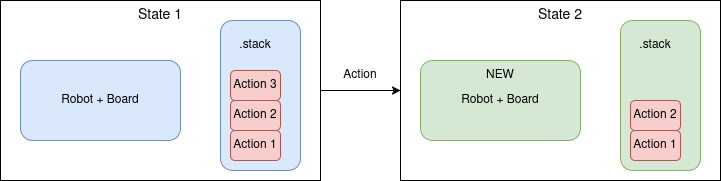
\includegraphics[width=0.8\textwidth]{action_game.png}
    \caption{Illustration d'un game based action}
    \label{fig:action_game}
\end{figure}

Pour écrire cette action nous définissons le constructeur \textbf{actionGame} qui convertit un action game (turn, move forward) en une action, c’est-à-dire additionne le dépilement du stack. Nous pouvons ajouter une condition aussi sur robot, si elle est fausse, on dépilera sans faire action game.
\\

Un \textit{action call} est une action qui dépile l'action (pour pas répéter) et empile les actions de function dans le bon ordre.

\begin{figure}[H]
    \centering
    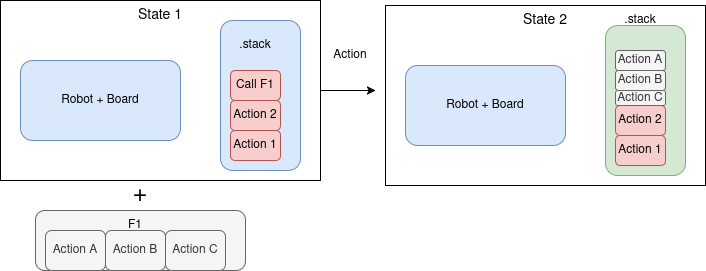
\includegraphics[width=0.8\textwidth]{action_call.png}
    \caption{Illustration d'un call action}
    \label{fig:action_call}
\end{figure}

Nous définissons le constructeur \textbf{actionFunct} qui convertit un function en action en dépilant le call et en empilant tous les action en appliquant \texttt{.reduce((acc: Stack<Action>, curr: Action) => cons(curr, acc), stackCall)} à function, c'est-à-dire on applique un algorithme \textit{folder} avec une fonction qui concatène avec l'action current au stack accumulateur, avec pour stack initial le stack dont action call à été dépilé (et un call stack expliqué plus tard).

Remarquez que l’ordre des actions sur la pile. Comme illustré par la figure \ref{fig:action_call}, on veut avoir l’action A en head par la logique de récursivité et call stack, or il serait en $3^{eme}$ position en empilant normalement. Pour cela nous créons une copie de function avec l'ordre des actions inversés avant d'appliquer le folder.

\subsection{Conditions de fin de partie}

Les condition de fin de partie sont le stack être vide \texttt{istackIsEmpty(aState.stack)}, avoir gagné \texttt{isWin(aState.board)}, l’agent être tombé \texttt{robotIsFell(aState.robot)} ou avoir un \textit{overstack} \texttt{isOverStack(aState.stack)}.

Cette dernière condition mérite une attention particulière. Robozzle autorise les fonctions récursives : une fonction peut s'appeler elle-même indéfiniment, provoquant une croissance infinie de la pile d'exécution. Pour détecter ce cas, le type \textit{Stack<T>} maintient un attribut \texttt{nb} qui comptabilise le nombre d'appels de fonctions effectués. Cet attribut est incrémenté exclusivement par l'opération \textbf{call(action, Stack<Action>)}, méthode similaire à \texttt{cons} mais tel que \texttt{call(action, stack).nb = stack.nb + 1}, contrairement \texttt{cons(action, stack).nb = stack.nb}.

\texttt{call} est utilisée dans \texttt{actionFunct} pour le premier empilement avant \texttt{.reduce(...)}. Lorsque \texttt{nb} dépasse 50, \textbf{isOverStack} est vérifiée et la partie se termine. Ce mécanisme permet d’interrompre toute exécution divergente.

\begin{figure}[H]
    \centering
    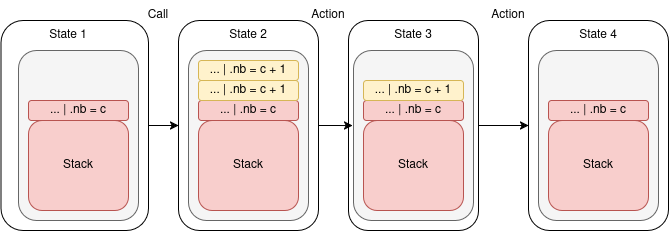
\includegraphics[width=0.6\textwidth]{nb_call.png}
    \caption{Illustration de l'attribut .nb dans un call}
    \label{fig:nb_call}
\end{figure}

\`A noter que quand toutes les actions liées à un call sont dépiler alors stack.nb reviens à .nb d’avant car les stacks ne sont pas modifiables comme illustré par la figure \ref{fig:nb_call}.

En combinant tout, nous avons:

\begin{figure}[H]
\centering
\begin{lstlisting}[language=, basicstyle=\ttfamily\small, frame=single, breaklines=true, captionpos=b]
function actionFunct(aFunctTrunk: () => Funct, cond?: (g: Robot) => boolean): Action {
  return (aState: State) => {
    // creation d'une fonction d'action d'ordre inversee
    const aFunct = aFunctTrunk().slice().reverse();
    // Si condition en robot vrai alors faire call
    if (cond === undefined || cond(aState.robot)) {
      
      // Fonction pour marquer call en stack
      // Avant d'appeller on depile action call
      const stackCall =
        (aFunct.length > 0)
          ? call(aFunct[0], tail(aState.stack))
          : tail(aState.stack);

      // Creation d'un nouveau tableau en empilant toutes 
      // action de function dans call       
      const stackNew = aFunct.
        slice(1).
        reduce((acc: Stack<Action>, curr: Action) => cons(curr, acc), 
               stackCall);

      // Retourner nouvel state
      return {
        robot: aState.robot,
        board: aState.board,
        stack: stackNew
      };
    } else {
      // Sinon on depile action call
      return {
        robot: aState.robot,
        board: aState.board,
        stack: tail(aState.stack)
      };
    }
  };
\end{lstlisting}
\caption{Algorithme du constructeur \texttt{actionFunct}}
\label{code:action_call_cons}
\end{figure}

Il y a une chose qu'on a pas expliqué, c'est a troncatrure \texttt{aFunctTrunk: () => Funct} dont nous allons expliquer dans la prochaine partie.

